\documentclass[tikz,border=10pt]{standalone}
\usepackage{tikz}
\usepackage{xcolor}
\usetikzlibrary{positioning,shapes.geometric,arrows.meta,shadows,decorations.pathreplacing,fit,calc}

% Define colors based on professional NASA/ESA style
\definecolor{primary}{RGB}{0,51,102}      % Dark blue
\definecolor{secondary}{RGB}{0,102,153}   % Medium blue  
\definecolor{accent}{RGB}{204,229,255}    % Light blue
\definecolor{warning}{RGB}{255,153,51}    % Orange
\definecolor{success}{RGB}{51,153,102}    % Green
\definecolor{neutral}{RGB}{102,102,102}   % Gray
\definecolor{background}{RGB}{248,249,250} % Light gray background

\begin{document}

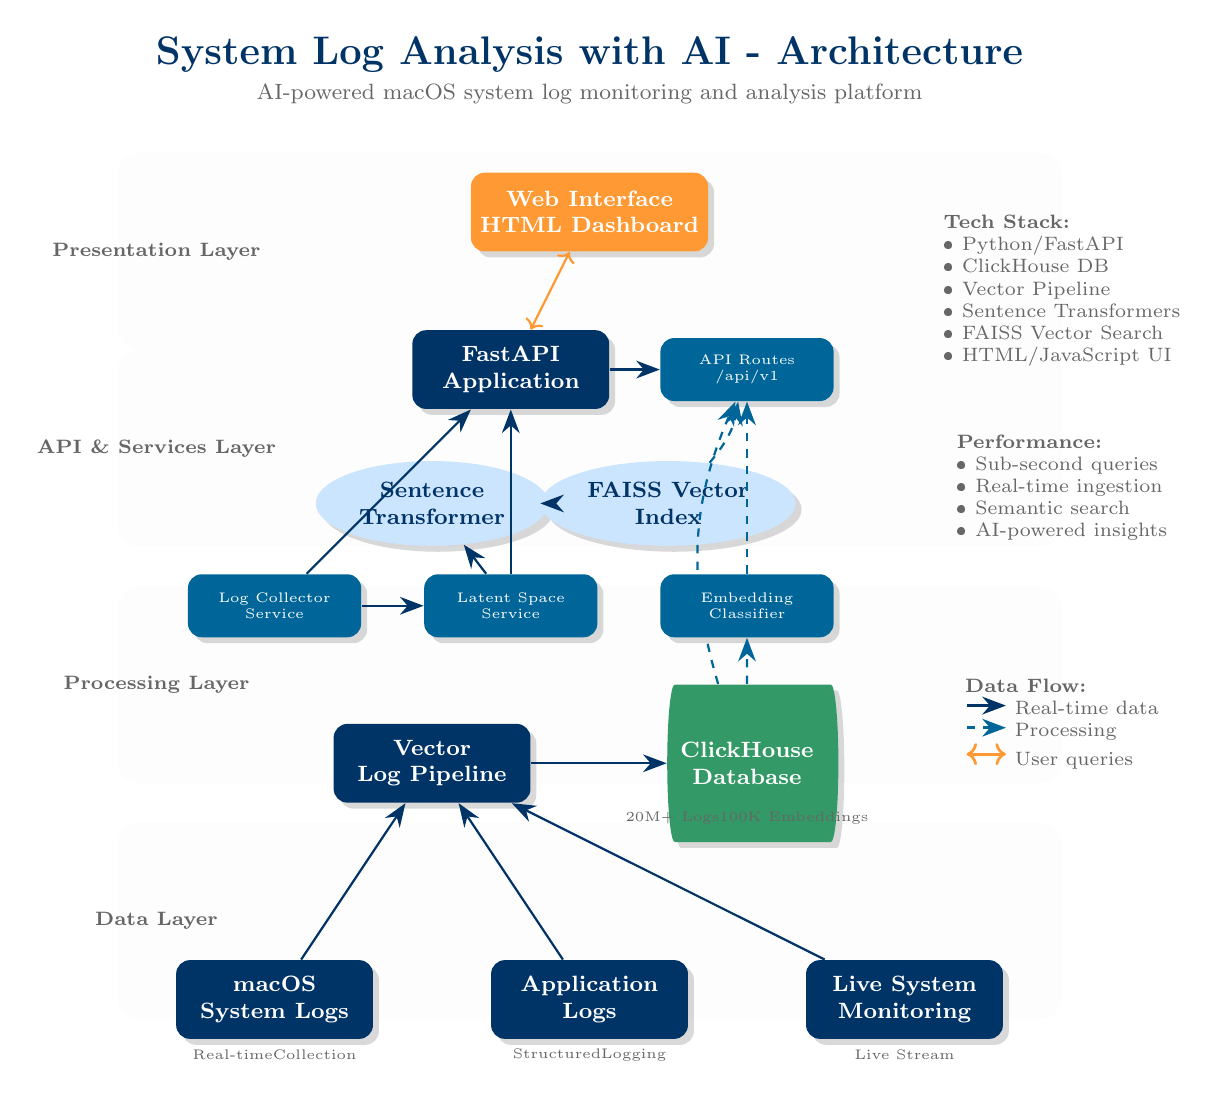
\begin{tikzpicture}[
    % Node styles
    system/.style={rectangle, rounded corners=5pt, fill=primary, text=white, 
                   minimum width=2.5cm, minimum height=1cm, align=center, font=\footnotesize\bfseries,
                   drop shadow={opacity=0.3}},
    service/.style={rectangle, rounded corners=5pt, fill=secondary, text=white,
                    minimum width=2.2cm, minimum height=0.8cm, align=center, font=\tiny,
                    drop shadow={opacity=0.3}},
    database/.style={cylinder, fill=success, text=white, minimum width=2cm, minimum height=1.2cm,
                     align=center, font=\footnotesize\bfseries, aspect=0.25,
                     drop shadow={opacity=0.3}},
    interface/.style={rectangle, rounded corners=5pt, fill=warning, text=white,
                      minimum width=2.5cm, minimum height=1cm, align=center, font=\footnotesize\bfseries,
                      drop shadow={opacity=0.3}},
    ai/.style={ellipse, fill=accent, text=primary, minimum width=2.5cm, minimum height=1cm,
               align=center, font=\footnotesize\bfseries, drop shadow={opacity=0.3}},
    % Arrow styles
    dataflow/.style={-{Stealth[length=3mm]}, thick, color=primary},
    process/.style={-{Stealth[length=3mm]}, thick, color=secondary, dashed},
    query/.style={<->, thick, color=warning},
    % Background styles
    layer/.style={rectangle, rounded corners=8pt, fill=background, opacity=0.3, 
                  minimum width=12cm, minimum height=2.5cm}
]

% Background layers
\node[layer] (data_layer) at (0, -4.5) {};
\node[layer] (processing_layer) at (0, -1.5) {};
\node[layer] (api_layer) at (0, 1.5) {};
\node[layer] (ui_layer) at (0, 4) {};

% Layer labels
\node[font=\scriptsize\bfseries, color=neutral] at (-5.5, 4) {Presentation Layer};
\node[font=\scriptsize\bfseries, color=neutral] at (-5.5, 1.5) {API \& Services Layer};
\node[font=\scriptsize\bfseries, color=neutral] at (-5.5, -1.5) {Processing Layer};
\node[font=\scriptsize\bfseries, color=neutral] at (-5.5, -4.5) {Data Layer};

% Data Sources (bottom layer)
\node[system] (macos_logs) at (-4, -5.5) {macOS\\System Logs};
\node[system] (app_logs) at (0, -5.5) {Application\\Logs};
\node[system] (live_logs) at (4, -5.5) {Live System\\Monitoring};

% Data Processing Layer
\node[system] (vector) at (-2, -2.5) {Vector\\Log Pipeline};
\node[database] (clickhouse) at (2, -2.5) {ClickHouse\\Database};

% Log Processing Services
\node[service] (log_collector) at (-4, -0.5) {Log Collector\\Service};
\node[service] (latent_space) at (-1, -0.5) {Latent Space\\Service};
\node[service] (embedding_classifier) at (2, -0.5) {Embedding\\Classifier};

% AI/ML Components
\node[ai] (sentence_transformer) at (-2, 0.8) {Sentence\\Transformer};
\node[ai] (faiss_index) at (1, 0.8) {FAISS Vector\\Index};

% API Layer
\node[system] (fastapi) at (-1, 2.5) {FastAPI\\Application};
\node[service] (api_routes) at (2, 2.5) {API Routes\\/api/v1};

% User Interface
\node[interface] (web_interface) at (0, 4.5) {Web Interface\\HTML Dashboard};

% Data flow arrows
\draw[dataflow] (macos_logs) -- (vector);
\draw[dataflow] (app_logs) -- (vector);
\draw[dataflow] (live_logs) -- (vector);

\draw[dataflow] (vector) -- (clickhouse);

\draw[dataflow] (log_collector) -- (latent_space);
\draw[dataflow] (latent_space) -- (sentence_transformer);
\draw[dataflow] (sentence_transformer) -- (faiss_index);

\draw[process] (clickhouse) -- (embedding_classifier);
\draw[process] (embedding_classifier) -- (api_routes);

\draw[dataflow] (log_collector) -- (fastapi);
\draw[dataflow] (latent_space) -- (fastapi);
\draw[dataflow] (fastapi) -- (api_routes);

\draw[query] (web_interface) -- (fastapi);

% Additional connections
\draw[process] (clickhouse) to[bend left=20] (api_routes);
\draw[process] (faiss_index) to[bend right=15] (api_routes);

% Data volume annotations
\node[font=\tiny, color=neutral] at (-4, -6.2) {Real-time\\Collection};
\node[font=\tiny, color=neutral] at (0, -6.2) {Structured\\Logging};
\node[font=\tiny, color=neutral] at (4, -6.2) {Live Stream};

\node[font=\tiny, color=neutral] at (2, -3.2) {20M+ Logs\\100K Embeddings};

% Technology stack annotations
\node[font=\scriptsize, color=neutral, align=left] at (6, 3.5) {
    \textbf{Tech Stack:}\\
    • Python/FastAPI\\
    • ClickHouse DB\\
    • Vector Pipeline\\
    • Sentence Transformers\\
    • FAISS Vector Search\\
    • HTML/JavaScript UI
};

% Performance metrics
\node[font=\scriptsize, color=neutral, align=left] at (6, 1) {
    \textbf{Performance:}\\
    • Sub-second queries\\
    • Real-time ingestion\\
    • Semantic search\\
    • AI-powered insights
};

% Data flow legend
\node[font=\scriptsize, color=neutral, align=left] at (6, -2) {
    \textbf{Data Flow:}\\
    \tikz{\draw[dataflow, line width=1pt] (0,0) -- (0.5,0);} Real-time data\\
    \tikz{\draw[process, line width=1pt] (0,0) -- (0.5,0);} Processing\\
    \tikz{\draw[query, line width=1pt] (0,0) -- (0.5,0);} User queries
};

% Title
\node[font=\Large\bfseries, color=primary] at (0, 6.5) {System Log Analysis with AI - Architecture};
\node[font=\footnotesize, color=neutral] at (0, 6) {AI-powered macOS system log monitoring and analysis platform};

\end{tikzpicture}

\end{document}
